\chapter{Grundlagen}

\section{SAP Customer Connection Programm}
%Wie unterscheide ich zwischen Ablauf und dem eigentlichen Programm

Um die Kundenzufriedenheit in Bezug zu den aktuellem \ac{plm} Applikationen zu steigern, gibt es seit Oktober 2017 das Customer Connection Programm, welches dem Kunden ermöglicht, Verbesserungsvorschläge für bestehende Softwarelösungen einzureichen und die dafür entwickelten Lösungen bereits vor offiziellem Release zu testen.\autocite[Vgl.][]{NoteCCP2021}

Das Programm richtet sich gezielt an SAP-Kunden, die bereits SAP On-Premise Lösungen benutzen, um gemeinsam mit dem Kunden neue Funktionalitäten zu erarbeiten. \autocite[Vgl.][]{CIP2021} Die Kunden können die bereits eingebrachten Vorschläge auf der Website des Customer Connection Programms einsehen und haben die Möglichkeit, für Vorschläge abzustimmen.

Sobald fünf Kunden einen Vorschlag unterstützen, wird die Umsetzungsrelevanz von einem SAP Projektteam evaluiert. Bei der Betrachtung spielen vor allem die Wichtigkeit des Vorschlags für andere Kunden, die Durchführbarkeit und die Wirtschaftlichkeit eine große Rolle. Für die Machbarkeit eines Vorschlags sind neben der Komplexität und Schwierigkeit einer Anpassung auch die verfügbaren Ressourcen von Bedeutung. Besonders gut bewertete Vorschläge werden kurzfristig, weniger interessante Kundenwünsche später realisiert oder abgelehnt. Wenn ein Kundenwunsch schon in ähnlicher Form implementiert ist, kann auch dies zur Ablehnung führen.\autocite[Vgl.][]{CCP}
\newpage
%3 Phasen mit 2 Calls in der Collect Phase
Das Programm sieht einen jährlichen Projektzyklus mit einer Gesamtlaufzeit von fünf Quartalen vor, der in verschiedene Phasen unterteilt wird.\autocite[Vgl.][]{NoteCCP2021} Zu Beginn können Kunden in der Collect Phase eigene Vorschläge einreichen und außerdem die Wünsche anderer Kunden befürworten. Je mehr Stimmen ein Vorschlag bekommt, desto wahrscheinlicher wird dessen Umsetzung. Auf die Collect Phase folgt die Selection Phase mit der Evaluierung der Kundenwünsche. Bei Fragen wird mit dem Kunden Rücksprache gehalten. Nach der erfolgreichen Umsetzung der Kundenwünsche werden während der Delivery Phase die fertigen Lösungen in Form von Hinweisen an alle relevanten SAP-Kunden ausgeliefert. Abgeschlossen wird die Delivery Phase mit der Bereitstellung eines Supportpackages, dass alle Hinweise des Projektzyklus enthält.\autocite[Vgl.][]{CCP}

%Anschließend wird in der Delivery Phase den Kunden die qualifizierten VorsIn der dritten und letzten Phase wird mit den Kick-off calls begonnen. Hier werden den Kundem die Liste der qualifizierten Vorschläge präsentiert und der Startschuss für die Umsetzung gegeben. Nach der Umsetzung des Kundenwunsches wird in Phase 4 die Lösungen an die Kunden ausgeliefert und in Delivery calls vorgestellt. In Phase 5 werden die letzten Kundenwünsche abgeschlossen und der komplette Projektzyklus wird reflektiert. Abgeschlossen wird der Projektzyklus mit dem Final call.\autocite{NoteCCP2021}\autocite{CCP}






\section{SAP PLM}


Die SAP-Applikation \acl{plm} hilft Unternehmen bei der Administration und Kontrolle des gesamten Lebenszyklus eines Produktes. Dabei werden Funktionen von der Produktentwicklung, der Herstellung über die Qualitätssicherung bis hin zu der Instandhaltung und Entsorgung abgedeckt. In der Anwendung können alle produktbezogenen Informationen verwaltet, verfolgt und überprüft werden.\autocite[Vgl.][S.232-236]{SAP01}
%sowohl im Verlauf des Produkt- und Analysezykluses als auch im Verlauf der erweiterten Logistikkette intergriert. \autocite[Vgl.][S.5]{SAPTEC}
%\autocite[Vgl.][S.232-236]{SAP01} 

Die Applikation SAP \ac{plm} kann sowohl in eine \acl{s/4hana} als auch in eine SAP-Business-Suite mit einem klassischen \ac{erp}-System integriert werden. Beide Systemlandschaften sind Geschäftsanwendungs-Paketlösungen, die eine Sammlung von betriebswirtschaftlichen Anwendungen zur Verfügung stellen. Für das Verständnis der späteren Ausführungen ist in diesem Zusammenhang vor allen Dingen bedeutsam, dass die Business-Suite \acs{s/4hana} nur mit der SAP \ac{hana} Datenbank eingesetzt werden kann und bei der Business-Suite mit klassischem \ac{erp}-System auch andere Datenbanken verwendet werden können.\autocite[Vgl.][S.4]{SAPTEC}

%Brauch man das: Durch Integration in die Business Suite können über die bestehenden Lösungsansätze in der Produktentwicklung hinaus auch Kunden und Lieferanten in erweiterte Prozessketten der Produktentwicklung miteinbezogen werden.\autocite[Vgl.][S.236]{SAP01}}

%\autocite[Vgl.][S.4]{SAPTEC}
\newpage
SAP \ac{plm} wird über ein Web User Interface bedient, dass als \ac{plmwui} bezeichnet wird. Auf der webbasierten Benutzeroberfläche können zum Beispiel Stammdaten, die den Lebenszyklus eines Produkts betreffen, angezeigt und bearbeitet werden. Zum Durchsuchen von Datenbeständen ist die \ac{plmwui}-Suche an die Enterprise Search angebunden.









\section{Technische Grundlagen}

\subsection{Enterprise Search}

Die \acl{es} wird für die einfache Suche in Business-Anwendungen wie der \ac{plmwui}-Suche benutzt und ermöglicht einen einheitlichen und sicheren Echtzeitzugriff auf Unternehmensdaten und -informationen innerhalb und außerhalb eines Unternehmens. Von der \ac{es} können sowohl strukturierte Business-Objekte wie Materialien oder Stücklisten als auch unstrukturierte Daten wie zum Beispiel PDFs aus SAP-Systemen zurückgegeben werden.\autocite[Vgl.][]{NetWeaverES} 

In der SAP-Systemlandschaft ist die Enterprise Search an den SAP NetWeaver angebunden, der als Middleware zwischen den klassischen Business-Anwendungen wie einem \ac{erp}-System und der Datenbank liegt.\autocite[Vgl.][S.13-15]{SAPTEC} Der SAP NetWeaver ist die Plattform für SAP-Geschäftsanwendungen und ermöglicht die Entwicklung, Bereitstellung und Verwaltung von SAP und nicht SAP Anwendungen in heterogenen IT-Landschaften.\autocite[Vgl.][S.8]{SAP01}


\begin{comment}
Der SAP NetWeaver ist die Plattform für SAP Geschäftsanwendungen und ermöglicht die Entwicklung, die Bereitstellung und die Verwaltung von SAP und nicht SAP Anwendungen in  heterogenen IT-Landschaften.\autocite[Vgl.][S.8]{SAP01} Als Technologie-Basis liegt SAP NetWeaver zwischen den klassischen Business-Anwendungen wie einem \ac{erp} System und der Datenbank.\autocite[Vgl.][S.24]{SAPTEC}

Als Technologie-Basis fungiert SAP NetWeaver als Mid-Wear und stellt die Kommunikation zeischen Anwendungen und Datenbank sicher.\autocite[Vgl.][S.24]{SAPTEC}


Jede dieser Business-Anwendungen kann die \ac{es} für die einfache Suche nutzen, um einen einheitlichen und sicheren Echtzeitzugriff auf Unternehmensdaten und -informationen innerhalb und außerhalb eines Unternehmens zu erlangen. Von der \ac{es} können sowohl strukturierte Business-Objekte wie Materialien oder Kundenaufträge als auch unstrukturierte Daten wie zum Beispiel PDFs aus SAP-Systemen zurückgegeben werden.\autocite[Vgl.][]{ES} 
\end{comment}



Beim Betreiben der \acl{es} wird zwischen zwei verschiedenen Suchabläufen unterschieden, die davon abhängen, ob der Kunde eine SAP \ac{hana} Datenbank oder einen anderen Suchdatenprovider nutzt. Bei den Kunden, die sich die Verbesserung gewünscht haben, kommen beide Varianten vor, weswegen nachfolgend beide Modelle vorgestellt werden.\autocite[Vgl.][]{ESV}

Der Betrieb der \acl{es} mit SAP \ac{hana} als Datenbank ermöglicht direkten Suchzugriff auf die in SAP \ac{hana} abgelegten Geschäftsdaten. Der Einsatz von weiteren Suchtechnologien ist hier nicht erforderlich.\autocite[Vgl.][]{ESV}

Beim Verwenden eines anderen, in der \ac{pam} gelisteten Suchdatenproviders ist der Anschluss der \ac{trex} erforderlich, um den fremden Suchdatenprovider im SAP System durchsuchen zu können.\autocite[Vgl.][]{ESV} 

Die Abbildung \ref{fig:ESHANA} zeigt, wie Suchanfragen bei der Anbindung von SAP \ac{hana} ausgeführt werden.


\begin{figure}[h]
    \centering
    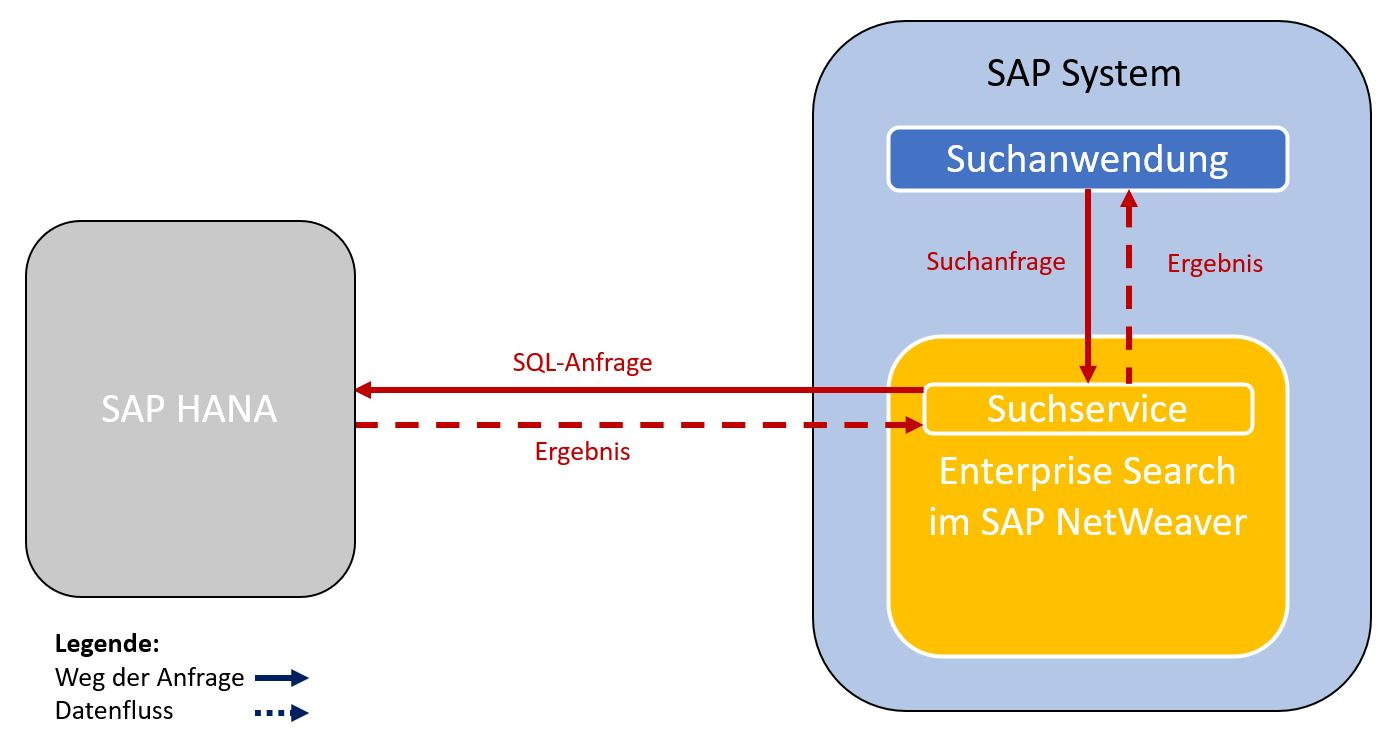
\includegraphics[width=1\textwidth]{img/ES_HANAselbst.JPG}
    \caption[ES Systemarchitektur mit SAP HANA]{ES Systemarchitektur mit SAP HANA\autocite{ESHANA}}
    \label{fig:ESHANA}
\end{figure}
\footnotetext{Vgl. eigene Darstellung angelehnt an: \textit{SAP Help Portal: ES Architektur der SAP-HANA basierten Variante 1} 2021.}

Zur Auswertung wird die Anfrage der Suchanwendung von der \ac{es} in ein \acs{sql}-Statement übersetzt.
\acs{sql} steht für Structured Query Language und wird für die Kommunikation mit Datenbanken eingesetzt. SAP HANA verarbeitet die \acs{sql}-Anfrage und gibt das Suchergebnis über die \ac{es} an die Anwendung zurück.\autocite[Vgl.][]{ESHANA}

Die Abbildung \ref{fig:ESBWA} zeigt wie Suchanfragen bei der Anbindung eines gelisteten Suchdatenproviders unter Nutzung von \ac{trex} abgewickelt werden.


Die \ac{trex} basierte Variante der Enterprise Search sucht mithilfe eines sogenannten Such-Indexes, der mögliche Suchbegriffe mit Suchergebnissen verknüpft. Zur Bildung der Indizes werden die Daten vom Suchdatenprovider mithilfe der \ac{es} extrahiert und daraufhin von \ac{trex} zu Indizes klassifiziert. Die Indizes enthalten Informationen zu dem Inhalt, dem Bearbeitungsort und der Bearbeitungsart der extrahierten Daten. Nachteil des Verfahrens ist, dass die gebildeten Such-Indizes regelmäßig aktualisiert werden müssen und das Aktualisieren sehr zeitaufwendig sein kann.\autocite[Vgl.][]{ESBWA}

\begin{figure}[h]
    \centering
    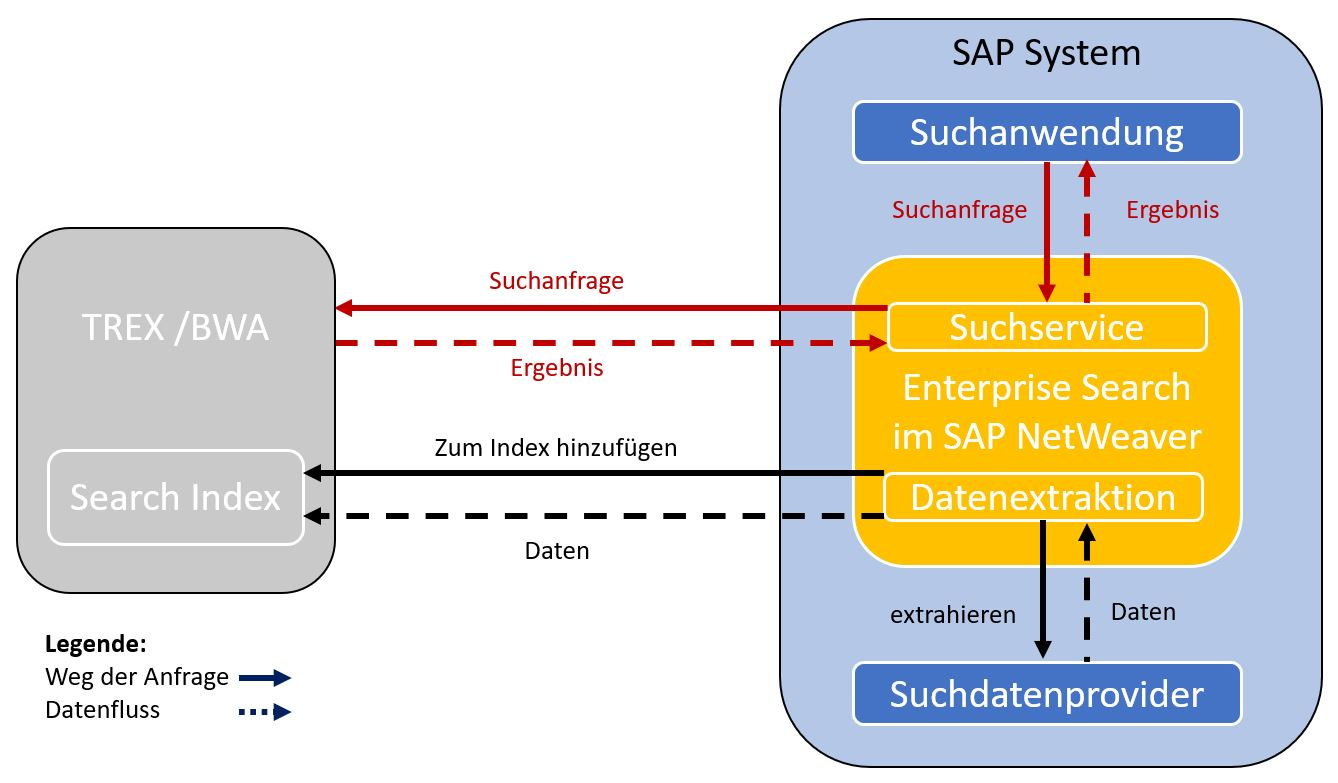
\includegraphics[width=1\textwidth]{img/ES_TREXselbstSuchdatenanbieter.JPG}
    \caption[ES Systemarchitektur mit TREX]{ES Systemarchitektur mit TREX\autocite[Vgl.]{ESBWA}}
    \label{fig:ESBWA}
\end{figure}
\footnotetext{Vgl. eigene Darstellung angelehnt an: \textit{SAP Help Portal: ES Architektur der TREX/BWA basierten Variante 1} 2021.}


\newpage
Wie in der Abbildung \ref{fig:ESBWA} zu erkennen ist, finden bei dem Verwenden eines anderen in der \ac{pam} gelisteten Suchdatenproviders zwei Abläufe statt. Bei der farblich schwarz dargestellten Extraktion und Indizierung der Daten, werden die Such-Indizes regelmäßig aktualisiert. Dazu prüft die \ac{es} die Daten zu eingeplanten Zeiten auf Änderungen. Falls sich der Datenbestand geändert haben sollte, werden die Veränderungen von \ac{trex} in die Such-Indizes aufgenommen.\autocite[Vgl.][]{ESBWA}

Die roten Pfeile zeigen den Verlauf einer Suchanfrage zur Laufzeit an. Beginnend bei der Suchanwendung wird die Anfrage von der \ac{es} an \ac{trex} weitergeleitet, um die Anfrage mit den Suchindizes abzugleichen. Die übereinstimmenden Inhalte werden anschließend als Ergebnis über die Enterprise Search an die Suchanwendung weitergegeben und dort auf der Suchoberfläche angezeigt. \autocite[Vgl.][]{ESBWA}


\begin{comment}
Zum einen das in Schwarz dargestellte extrahieren und indizierung der Daten und zum anderen der in Rot abgebildete Verlauf einer Suchanfrage zur Laufzeit. Teil der Indizierung ist das regelmäßige Aktualisieren der Such-Indizes. Dabei prüft die \ac{es} die Datenbestände zu eingeplanten Zeiten auf Änderungen und gibt diese anschließend an \ac{trex} oder \ac{bwa} weiter. Diese nehmen die Änderungen in die Such-Indizes auf.

Zur Laufzeit werden die eintreffenden Suchanfragen nicht direkt an die Datenbank weitergegeben, sondern von der \ac{es} an \ac{trex}/\ac{bwa} weitergeleitet. Daraufhin wird die Suchanfrage mit den Suchindizes abgeglichen und die übereinstimmenden Inhalte als Suchergebnis an die Enterprise Search übertragen. Letztlich wird das Ergebnis von der \ac{es} an die Suchanwendung gesendet und der Benutzer bekommt die Ergebnisse auf der Suchoberfläche angezeigt. \autocite[Vgl.][]{ESBWA}
\end{comment}
Somit ist die Enterprise Search in der Lage, Suchanfragen unabhängig von der Systemarchitektur zu verarbeiten und ein passendes Suchergebnis zurückzugeben.



\subsection{ABAP}
%alternativer Start: ABAP, was mittlerweile für Advanced Business Applikation Programming steht,ist eine von SAP entwickelte Programmiersprache zur Programmierung von kommerzielen Anwendungen im SAP Umfeld.

\acs{abap} ist die Kurzform für Advanced Business Applikation Programming und wurde zur Programmierung von kommerziellen Anwendungen im SAP-Umfeld entwickelt.
Die SAP eigene Programmiersprache gehört zu den \ac{4gl}-Sprachen und bietet dadurch viele Vorteile gegenüber elementaren Sprachen.\autocite[Vgl.][S.25]{KELLER2015}
Ein wesentlicher Unterschied von \acs{abap} zu vielen anderen Programmiersprachen ist, dass die Programme nach dem Speichern noch aktiviert werden müssen, bevor sie ausführbar sind.

\acs{abap} Programme bestehen aus einem globalen Deklarationsteil, indem die Variablen, die für das ganze Programm gültig sind, deklariert werden und einem prozeduralen Teil. Hier werden die Anweisungen, die anschließend sequenziell ausgeführt werden, implementiert.\autocite[Vgl.][S.92f]{KELLER2015} Erkennbar ist \acs{abap} insbesondere an den großgeschriebenen \acs{abap}-Schlüsselwörtern und dem Punkt am Ende jeder Befehlszeile. 

%Die Entwicklungsumgebung für ABAP Programme und alle ihre Komponenten ist die ABAP Workbench.
Eingesetzt wird \acs{abap} mithilfe der \acs{abap}-Workbench sowohl zur Entwicklung vollständig neuer Anwendungen als auch zur Erweiterung und Modifikation von SAP Standardanwendungen. Elementarer Bestandteil der \acs{abap}-Workbench, zu der eine Vielzahl von Werkzeugen zur \acs{abap}-Programmierung gehören, ist der \acs{abap}-Editor, mit welchem \acs{abap}-Programme angezeigt, geändert und ausgeführt werden können.\autocite[Vgl.][S.57,88f]{KELLER2015}

Ein wichtiges Element des \acs{abap}-Editors ist der \acs{abap}-Debugger, der die Untersuchung eines Programmcodes ermöglicht. Er eignet sich besonders gut, um die Logik des Quellcodes zu verstehen und Fehler im Programm zu finden, die die Ausführung behindern.\autocites[Vgl.][S.92-96]{S4D400}[S.87f]{GAHM2016} Beim Debuggen können zu Beispiel Rückschlüsse auf Fehler im Code durch das Anzeigen der aktuellen Werte der Variablen gezogen werden.



\subsection{Web Dynpro}
%Die WebDynpro Benutzungsoberfläche (UI) der Enterprise Search bietet einen zentralen Einstiegspunkt, um strukturierte und nicht strukturierte Daten Ihres Unternehmens aus verschiedenen Quellen mit einer einzigen Suche zu finden. \autocite{ES}
%WebDynpro steht für ... und ...
%Browser basiert , keine Installation
% (Die Anwendungen können in die Portalumgebung des SAP NetWeavers eingebunden oder von einem Browser angezeigt werden.)
%den Aufwand der Entwickler für die Erstellung leistungsfähiger Webanwendungen in einem strukturiertem Entwicklungsprozess zu minimieren. WenDynpro Anwendungen erleichtern
% Der von den Grundbausteinen generierte Quellcode wird als Web-Dynpro-Framework bezeichnet.

Die seit SAP NetWeaver 7.0 zur Verfügung stehende Web-Dynpro \acs{abap} Technologie ermöglicht die Entwicklung von \acs{abap} basierten Webanwendungen mit deklarativen Programmiertechniken. Ziel ist es, das Erstellen von \acp{ui} in der \acs{abap}-Workbench durch eine Auswahl von Grundbausteinen, die automatisch Quellcode generieren, zu erleichtern. Mit \acs{abap} Code lässt sich die zur Designzeit von Grundbausteinen aufgebaute Benutzeroberfläche für jede erforderliche Anwendungsfunktion erweiterten.\autocite[Vgl.][S.2f]{NET310}

Einer der Grundsätze der Web-Dynpro-Philosophie lautet: "Je weniger von Hand geschriebener Code, desto besser" \autocite[Vgl.][S.5]{NET310}. Das hat den großen Vorteil, dass iterative Programmieraufgaben, wie sie bei HTML und JavaScript auftreten, entfallen und folglich das Risiko auf Fehler im Programm minimiert wird.\autocite[Vgl.][S.2f]{NET310}

Web-Dynpro Anwendungen basieren auf dem Model-View-Controller Prinzip, damit die Geschäftslogik sauber von der Benutzeroberfläche getrennt werden kann. Das Prinzip teilt die zu erstellenden Programme in die Bereiche Model, View und Controller auf. \autocite[Vgl.][S.15]{NET310}

Der Model-Bereich stellt die Anwendungsdaten, auf die während der Laufzeit zugegriffen werden soll, zur Verfügung.\autocite[Vgl.][S.734]{KELLER2015}

Der View-Bereich repräsentiert den sichtbaren Teil der Anwendung und legt folglich das Design und die benötigten Web-Dynpro-Elemente fest.\autocite[Vgl.][S.15]{NET310}

Der Controller-Bereich ist für die Prozessierung der Daten zur Laufzeit verantwortlich und beinhaltet die Klassen und Methoden zur Datenverarbeitung.\autocite[Vgl.][S.734]{KELLER2015} 

\begin{figure}[h]
    \centering
    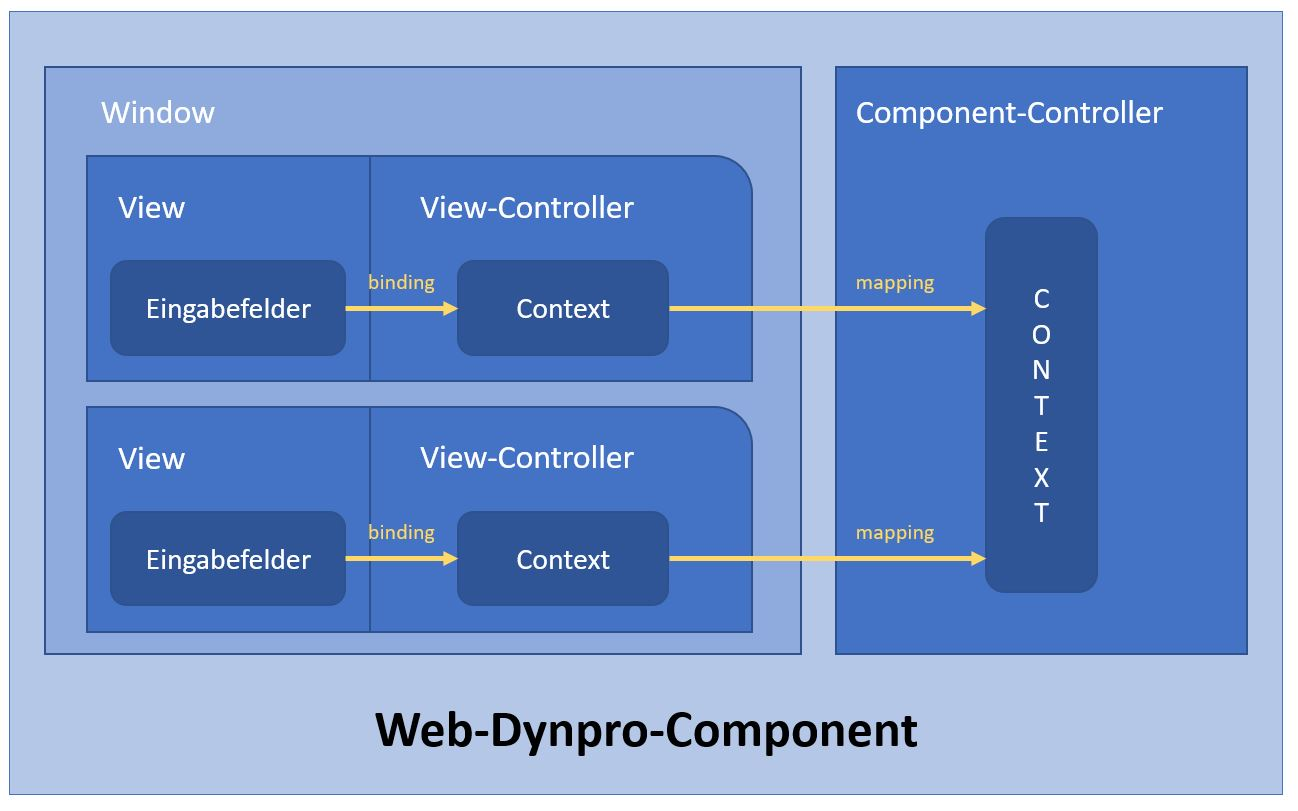
\includegraphics[width=1\textwidth]{img/WebDynpro_Componentselbst.JPG}
    \caption[Architektur eines Web-Dynpro-Components]{Architektur eines Web-Dynpro-Components\autocite[S.7]{NET310}}
    \label{fig:WebDynproComponent}
\end{figure}
\footnotetext{Vgl. eigene Darstellung angelehnt an: o.V. 2010, S.7.}


Der Rahmen einer jeden Web-Dynpro Anwendung ist der Web-Dynpro-Component. Wie in der Abbildung \ref{fig:WebDynproComponent} zu sehen, umschließt der Component als Container alle anderen Web-Dynpro-Entitäten.

%Den sichtbaren Teil einer Web-Dynpro Anwendung repräsentiert die View mit seinem Layout, dass unteranderem Eingabefelder, Labels und Drucktasten enthält, und mit dem View Designer grafisch gestaltet werden kann.

%Zu den UI bezogenen Entitäten gehören Windows und Views. Eine View ist ein Objekt ohne Schnittstelle zu "der Welt außerhalb der Component" \autocite[S.740]{KELLER2015}, weswegen es zunächst in ein Web-Dynpro-Window eingebunden werden muss. Jeder View besitzt zusätzlich zu dem Layout einen View-Controller, welcher eigene Methoden und Context-Elemente besitzt, auf welche nur der View selbst zugreifen kann. Dieser Controller steuert die View spezifische Ablauflogik, wie zum Beispiel die für die Ereignisbehandlung vorgesehenen Methoden, die nach dem Anklicken einer Schaltfläche aufgerufen werden.\autocite[Vgl.][S.738]{KELLER2015}

Der View repräsentiert dabei den sichtbaren Teil einer Web-Dynpro-Component. Das Layout des Views, das unter anderem Eingabefelder, Labels und Drucktasten enthält, kann mit dem View Designer grafisch gestaltet werden. Zusätzlich gehört zu jedem View auch ein View-Controller, auf dessen Methoden und Context-Elemente nur der View selbst zugreifen kann. Dieser Controller steuert die View spezifische Ablauflogik wie zum Beispiel die für die Ereignisbehandlung vorgesehenen Methoden, die nach dem Anklicken einer Schaltfläche aufgerufen werden.\autocite[Vgl.][S.738]{KELLER2015}

Aufgrund der Tatsache, dass der View selbst keine Schnittstelle zur "Welt außerhalb der Component hat"\autocite[S.740]{KELLER2015}, muss er zur Verwendung in ein Web-Dynpro-Window eingebunden werden. Dieses bestimmt als \ac{ui}-Container, in welcher Anordnung welche Views im Browser angezeigt werden sollen. Dabei kann ein Window eine beliebige Anzahl an Views enthalten und ein View in eine beliebige Anzahl von Windows eingebettet sein. \autocite[Vgl.][S.740]{KELLER2015}

Der in der Abbildung \ref{fig:WebDynproComponent} rechts zu sehende Component-Controller steuert die Funktionen des gesamten Components. Er ist als zentraler Controller für alle anderen Controller im Component erreichbar und enthält daher alle öffentlichen Methoden der Web-Dynpro-Component. Im Gegensatz zu den View-Controllern hat er allerdings keine visuelle Schnittstelle. \autocite[Vgl.][S.45f]{NET310}

Zu jedem Component- und View-Controller gehört jeweils ein Context, der die für die Methoden des Controllers benötigten Daten als Context-Attribute bereitstellt und unter Knoten gruppiert.\autocite[Vgl.][S.61f]{HOFFMANN2006}

%Damit die Eingaben auf der Benutzeroberfläche zu jedem Zeitpunkt mit den Context-Attributen übereinstimmen, werden die \ac{ui}-Elemente mit den Context-Attributen verknüpft. In Web-Dynpro Umfeld wird diese Verbindung als Data-Binding bezeichnet.
\newpage
Um die Eingaben auf der Benutzeroberfläche an die Methoden der Controller weitergeben zu können, müssen die entsprechenden \ac{ui}-Elemente mit den dazugehörigen Context-Attributen verknüpft sein. Diese Verbindung wird als Data-Binding bezeichnet. Zweck des Bindings ist es, den Wert des \ac{ui}-Elements zu jedem Zeitpunkt mit dem Wert des dazugehörigen Context-Attributes zu synchronisieren.\autocite[Vgl.][S.752]{KELLER2015}

Damit die View-Controller untereinander Attributwerte austauschen können, werden alle Attribute des View-Contextes auf gleichnamige Attribute im Component-Controller-Context gemappt. Ändert sich dann ein Wert eines Attributes im View-Controlller, beispielsweise durch die Eingabe eines Benutzers, werden dadurch neben den Context-Attributen des Views auch die referenzierten Attribute im Component-Controller aktualisiert.\autocite[Vgl.][S.8]{NET310}

%Jeder Web-Dynpro-Component hat außerdem als Bindeglied zwischen der Datenbank und den Controllern eine \ac{ui}-Struktur. Damit die Die \ac{ui}-Struktur legt mit vordefinierten Typen fest, wie die in der Suchoberfläche eingegebenen Daten auszusehen haben.
%Jeder Web-Dynpro-Component hat außerdem eine \ac{ui}-Struktur, die mit vordefinierten Typen festlegt, wie die in der Suchoberfläche eingegeben Daten auszusehen haben, damit die dazugehörigen Daten in der Datenbank gefunden werden können. Somit ist eine \ac{ui}-Struktur das Bindeglied zwischen Datenbanktabellen und dem Component-Controller. \change{Marco fragen}

%Durch das Data-Binding, das Context-Mapping und das Verwenden einer \ac{ui}-Struktur können die im \ac{ui} eingegebenen Daten an unterschiedliche Views, Controller und Datenbanktabellen transportiert werden. 

Das Kapseln von visuellen und programmtechnischen Web-Dynpro-Entitäten ermöglicht, dass jeder Web-Dynpro-Component in anderen Components wiederverwendet werden kann.\autocite[Vgl.][S.5]{NET310} 
%Jeder Component hat ein Interface, dass die Schnittstelle zu anderen Komponenten darstellt. Fremde Methoden und Ereignisse können im Interface-Controller bereitgestellt und mit dem visuellen Interface können auch visuelle Entitäten in die Windows anderer Components eingebunden werden.
So können in der Praxis für wiederkehrende Aufgaben wie das Anlegen eines Auftrags oder das Verwalten einer Adresse generische Components angelegt werden, die anschließend als Bausteine in andere Web-Dynpro-Anwendungen eingebettet werden. 

